% Introduction
\chapter{Introduction}
\vspace{-1cm}

Modern technologies --- including catalysts, high-strength alloys, high-efficiency phosphors, lasers, and magnets --- are dependent upon the unique properties of the rare earth elements (REE) for their efficacy of operation.
However, global REE material-flows are prone to complex environmental, technical, and geopolitical forces on both the supply- and demand side.
Development of economically-viable technologies for the extraction of the REE and other critical materials from unconventional sources (such as geothermal fluids, oil and gas produced waters, or coal combustion residuals) has great potential value to: generate a consistent domestic supply of materials critical to green energy and defense technologies; valorize high-volume wastes or low-value industrial byproducts; and avoid environmental impacts from primary REE mining.

\section{What are rare earth elements?}
The REE constitute much of Group 3 of the periodic table, a group of 16 transition metals, including the lanthanide series (La to Lu, excluding Pm), Yttrium (Y) and Scandium (Sc).
The ``rare'' moniker stems from their initial isolation from uncommon mineral phases in the 18th and 19th century \citep{CastorHedrick},
though the natural abundance of REE in the earth's crust range from 0.52 parts per million (ppm) to 41.5 ppm, in the same range as Pb or Sn and exceeding the natural, crustal abundance of Ag and Hg \citep{CRC}.

In the natural sciences, predictable thermodynamic differences between the REE make these elements uniquely capable tools for interpreting natural geologic and chemical processes \citep{Murray_Geol_1990, Laveuf_Geoderma_2009}.
Rare earth lithogeochemistries have long been used to infer depositional environments of geologic strata \citep{Murray_Geol_1990, PAAS, Hanson_AREPS_1980}.
Similarly, REE serve as benign analogs to the transuranic actinide series for nuclear waste disposal studies \citep{Krauskopf_CG_1986, Millero_GCA_1992};
as potential markers of regional authenticity for high value exported food products such as wine, pumpkin-seed oil, and olive oil \citep{Jakubowski_FJAC_1999, Joebstl_FC_2010, Farmaki_AL_2012};
and for studying mixing and metal cycling in the oceans \citep{DeBaar_Nature_1983, Elderfield_PTRS_1988}.

Many of the same properties that yield the unique and predictable geochemistry of the REE have lead to their use in more consumer products than nearly any other element group \citep{CastorHedrick, Graedel_PNAS_2015}. In most applications, the performance of the REE is unmatched \citep{Ciacci_EST_2015, Nassar_JIE_2015}, making substitution (with more readily available/environmentally benign elements) undesirable.

Based on atomic number, the REE are segregated into light and heavy REE (LREE and HREE, respectively) with the division occurring between Eu and Gd \citep{CastorHedrick};
some studies further distinguish middle REE (MREE), though the specific elements are inconsistently defined between authors \citep{Hannigan_CG_2001, Tang_CG_2010, Choi_CG_2009}.
These ``weight'' distinctions allow for simplified description and quantification of the inter-element relationships, typically ratios of normalized concentrations, which are exploited in REE analysis.
Similarly, anomalies of certain REE --- due to redox lability for Ce and Eu \citep{Brookins_RMG_1989} and large anthropogenic emissions for Gd \citep{Bau_EPSL_1996} --- are used to interpret geochemical processes.
Y and Sc exhibit similar properties to the lanthanides and are thus included in the suite of REE with Y being most similar to HREE and Sc being most similar to LREE in solution \citep{Brookins_RMG_1989}. 

\section{What is the context of this study?}

The constantly increasing consumer products incorporating the REE, and the ensuing demand for these products, have established the REE as valuable global commodities.
Domestic demand in 2012 was 11,300 tons, while the global demand was more than 113,000 tons \citep{FrostSullivan_REEmarket}.
Much of that demand is a result of a booming green energies market.
In particular, the permanent magnets sector is expected to experience significant growth between 2013 and 2020.
High-efficiency generators used in turbines and electric motors require strong and light permanent magnets.
Currently, magnets using neodymium, praseodymium, and samarium (with dysprosium and terbium additives) are the strongest and lightest commercially available.

Even at the height of domestic REE production at Mountain Pass in CA (2012), the U.S. imported \$520MM worth of REE compounds, with nearly 40\% coming from China, in order to support a demand of 11,300 tons \citep{USGS_minyb_2012}.
A booming green energies industry fueled, and continues to fuel, both domestic and global demand, where the REE provide superior performance and efficiency compared to alternative materials \citep{Nassar_JIE_2015, Graedel_PNAS_2015}.
Sustained growth in these technologies is dependent on diversifying REE sources given projected supply shortages in the medium- to long-term.
Traditional mining of REE from ore deposits is unlikely to fulfill this demand for technical and economic reasons, especially in the US where traditional mining of REE is suspended.
China, the world's leading source of REE and primary supplier of global demand for many years (Figure~\ref{fig:world-REO-prod}, has indicated partial control of exports, or punitive tariffs, in the near future.
This emphasizes the need for REE separation and recovery from unconventional matrices, such as geothermal fluids or coal fly ash.

\begin{figure}[htbp]
\begin{center}
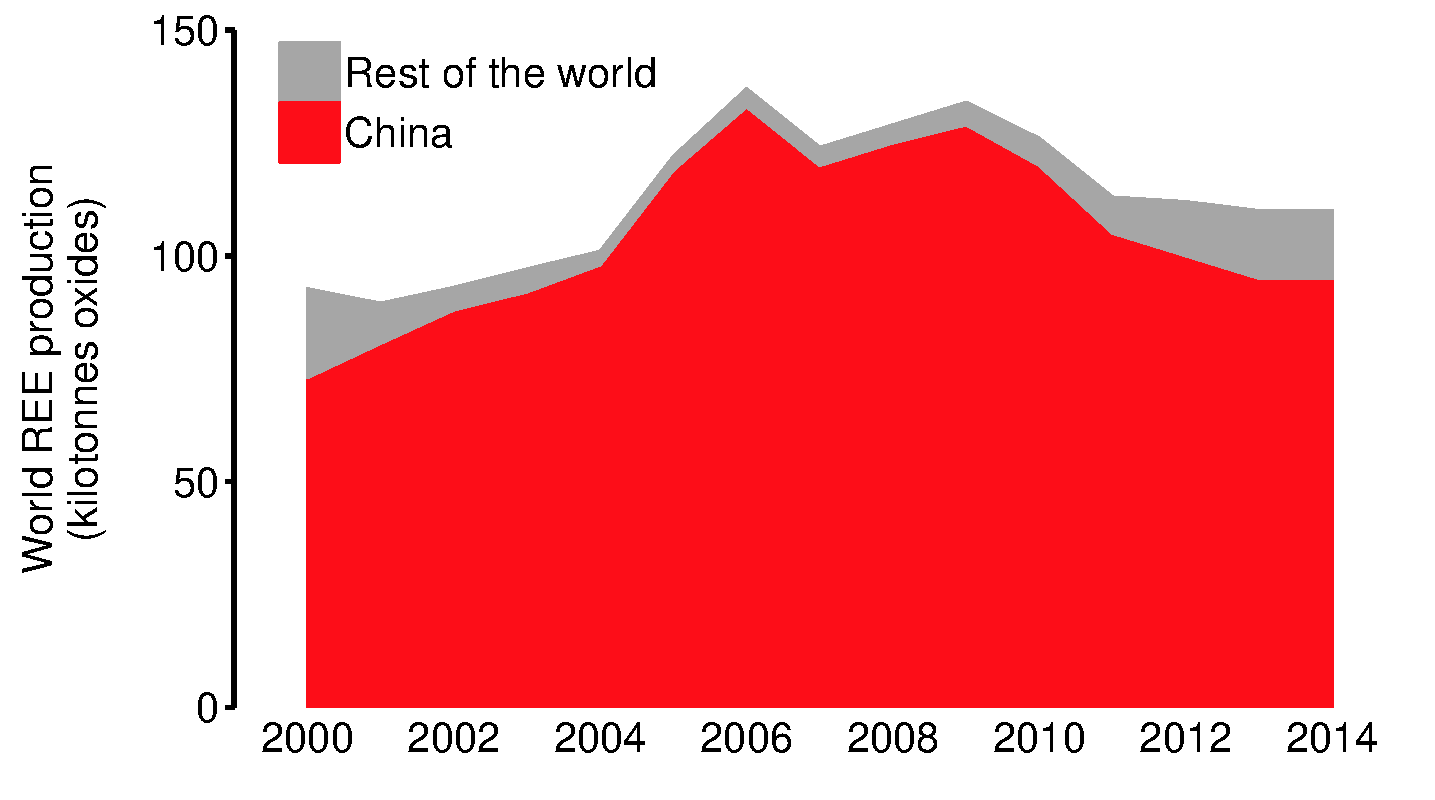
\includegraphics[width = 0.7\textwidth]{proposal_figures/World-REO-production.pdf}
\caption{Global, primary REE production, 2000-2014.
Data from \citet{USGS_commsumm}.}\label{fig:world-REO-prod}
\end{center}
\end{figure}

Global REE reserves are estimated at 130 million metric tons \citep{USGS_commsumm}, much of which is located in low-concentration deposits or ocean-floor manganese nodules, which are both extremely expensive to mine with current methods.
This limits the number of readily mineable REE deposits and, ultimately, our ability to increase REE supply \citep{JRC_2011, Alonso_EST_2012}.
Aqueous media such as brines or produced waters from geothermal energy, conventional oil/gas, and shale gas extraction operations are potentially significant, but unexplored sources of REE.

Presently, REE extraction is accomplished by traditional mining (e.g. open-pit) followed by chemically-, and energy-intensive element separations, which incur a significant environmental burden (Figure~\ref{fig:Zaimes-LCA}; \citep{Zaimes_SCE_2015}).
Even when present in ores at appreciable levels, REE are commonly commingled with radioactive thorium and uranium, which need to be safely separated and stored in addition to standard waste management associated with mining (e.g. tailings) \citep{Gupta_IMR_1992, Sprecher_EST_2014}.
Stringent environmental regulations, time-intensive processes, and expensive permits complicate the opening of new, domestic mines because of these inherent risks.
On this basis, projections expect that exploiting traditional REE sources to meet increasing demand will be a significant challenge.
In 2012, China was responsible for more than 95\% of the global REE supply \citep{USGS_commsumm}.
China also had the largest demand for REE, at 66\% of the total global demand \citep{USGS_commsumm}.
The US was the next largest consumer, at 10--15\% of the total demand.
In 2011, China announced a 35\% reduction in exports of REE, in an effort to meet their domestic needs \citep{USGS_minyb_2012}.
This created large instability in the REE market as there were no other major sources for REE \citep{Alonso_EST_2012, Chakmour_Elem_2012, Hatch_Elem_2012}.
China is expected to continue reduction of exports, through either quotas or tariffs, as a mean to reduce stress on its REE reserves \citep{FrostSullivan_REEmarket, USGS_commsumm}.

\begin{figure}[htbp]
\begin{center}
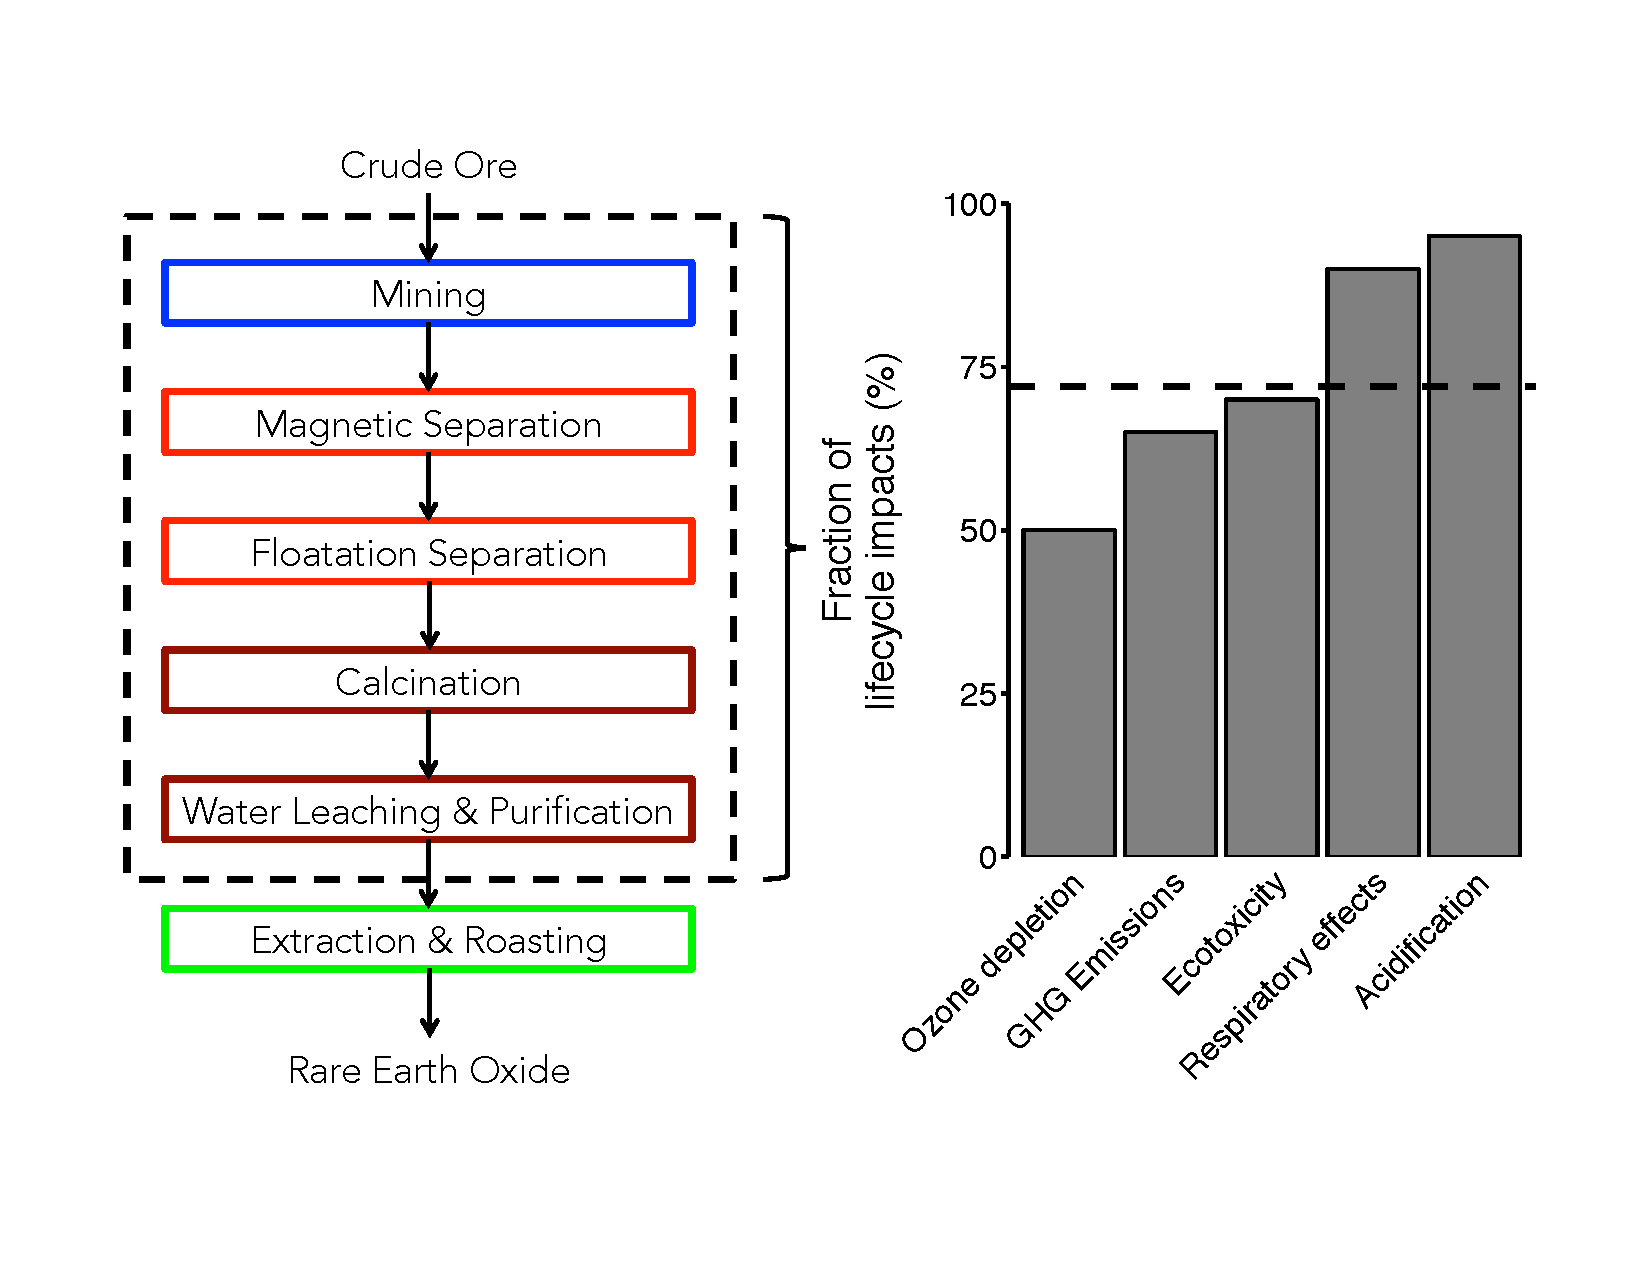
\includegraphics[width = \textwidth]{proposal_figures/Zaimes-LCA-schematic.pdf}
\caption{Traditional REE production flowsheet (left) and the associated fraction of lifecycle environmental impacts for the boxed boundary (right) using data from \citet{Zaimes_SCE_2015}.
Only selected impact categories are shown, however the dashed line (72\%) indicates the overall average across ten categories.}\label{fig:Zaimes-LCA}
\end{center}
\end{figure}

Primary mining effectively constitutes 100\% of the REE production worldwide \citep{Binnemans_JCP_2013, USGS_commsumm},
but interest in recovery of REE from end-of-life stocks (EOL), from unconventional resources, and from REE-containing industrial wastes has expanded rapidly in recent years \citep{Binnemans_JCP_2015}.
High volumes of REE are deployed in permanent magnets, while high-value REE are used in phosphors \citep{Hatch_Elem_2012},
making these products two primary targets for recycling from EOL products along with metal hydride batteries \citep{Binnemans_JCP_2013,Tunsu_Hydro_2015}.
REE are applied in many other products, but the REE content is dissipated in-use or rendered unrecyclable by current designs \citep{Ciacci_EST_2015}.
Ferrous shredder waste (where magnets could accumulate) is a promising potential resource for REE and other critical materials.
However, \citet{Bandara_JSM_2015} propose that recycling of ferrous shredder-waste would need to exceed 50\% in order to dampen Nd price volatility from recycling alone. The conclusion from these forecasts is the need for novel, alternative feedstocks \citep{Bandara_JSM_2015}.

\section{What are the goals of this study?}
This research seeks to address the potential for REE extraction and recovery from dilute aqueous sources.
This work is motivated by the desire to diversify REE sources, promote development of low-carbon energy sources, valorize industrial byproducts, and avoid the environmental disruption associated with primary REE mining.
A combination of a literature analysis, analytical method development, controlled experimentation, and statistical and geochemical modeling will be used to address these goals.

The three, specific objectives of this work and the related questions they were developed to answer are as follows:
\begin{enumerate}
	\item Determine REE abundance and trends in natural waters.
	\begin{itemize}
		\item	What is the natural variability of REE in aqueous media?
		\item	What quantitative methods exist for considering below detection limit values?
		\item	What is known about REE occurrence in brines?
		\item	What relationships between REE and bulk solution properties are important for REE fate and transport?
	\end{itemize}
	\item Develop efficient liquid-liquid extraction technique for separation of REE from hypersaline brines.
	\begin{itemize}
		\item	How are REE measured in aqueous samples?
		\item Will these techniques work for hypersaline, chemically complex brines?
		\item What are the limits of effectiveness for an LLE technique (with respect to brine composition)?
	\end{itemize}
	\item	Study the effects of ligand functionality and geometry on the partitioning behavior of the REE from brines to functionalized adsorbents
	\begin{itemize}
		\item	What ligands have high, aqueous-phase affinity for the REE?
		\item How does surface attachment affect the affinity of these ligands for the REE?
		\item What are the best performing ligands for REE recovery?
		\item How do these ligands perform under a range of aqueous conditions? 
	\end{itemize}
\end{enumerate}

The specific objectives of this work were developed to address gaps in the literature to date while building on the existing REE and functionalized adsorbent knowledge base. These objectives are meant to address application specific (i.e. REE recovery from geothermal brines) uncertainty as well as foster a more fundamental understanding of the REE systematics. The methods proposed to address these objectives are detailed in \S2.1-2.3.
